\documentclass[tikz,border=10pt]{standalone}
%% definition of the central band, just to show 
%% that in both configurations the same color is used
\newcommand{\colorband}[1][]{%
  \foreach \a in {0.2,0.6,...,4}
    \draw[line width=0.2cm,#1] (\a,1)--(\a,2);}
%% definition of the remaining part
\newcommand{\stripes}[1][]{%
  \foreach \b in {0,0.4,...,4}
    \draw[line width=0.2cm,#1] (\b,0)--(\b,3);}
\newcommand{\middlestripes}[1][]{%
  \foreach \b in {0.2,0.6,...,4}
    \draw[line width=0.2cm,#1] (\b,0)--(\b,1)(\b,2)--(\b,3);}
\begin{document}
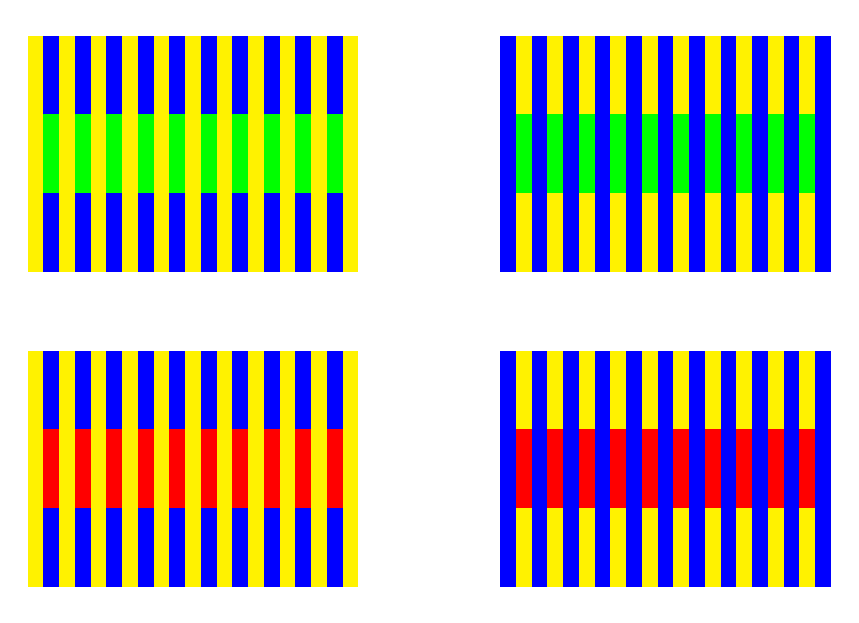
\begin{tikzpicture}
%% red band, orange and magenta perception
  \colorband[red]
  \stripes[yellow]
  \middlestripes[blue]
  \begin{scope}[xshift=6cm]
    \colorband[red]
    \stripes[blue]
    \middlestripes[yellow]
  \end{scope}
  \begin{scope}[yshift=4cm]
%% green band, lime and cyan perception
    \colorband[green]
      \stripes[yellow]
      \middlestripes[blue]
    \begin{scope}[xshift=6cm]
      \colorband[green]
      \stripes[blue]
      \middlestripes[yellow]
    \end{scope}
  \end{scope}
\end{tikzpicture}
\end{document}